\documentclass[12pt]{article}
% \usepackage[top=1in,left=1in, right = 1in, footskip=1in]{geometry}
\usepackage[top=1in,footskip=1in]{geometry}

\usepackage{graphicx}
\usepackage{xspace}
%\usepackage{adjustbox}

\usepackage{grffile}

\newcommand{\comment}{\showcomment}
%% \newcommand{\comment}{\nocomment}

\newcommand{\showcomment}[3]{\textcolor{#1}{\textbf{[#2: }\textsl{#3}\textbf{]}}}
\newcommand{\nocomment}[3]{}

\newcommand{\jd}[1]{\comment{cyan}{JD}{#1}}
\newcommand{\swp}[1]{\comment{magenta}{SWP}{#1}}
\newcommand{\bmb}[1]{\comment{blue}{BMB}{#1}}
\newcommand{\djde}[1]{\comment{red}{DJDE}{#1}}

\newcommand{\eref}[1]{Eq.~(\ref{eq:#1})}
\newcommand{\fref}[1]{Fig.~\ref{fig:#1}}
\newcommand{\Fref}[1]{Fig.~\ref{fig:#1}}
\newcommand{\sref}[1]{Sec.~\ref{#1}}
\newcommand{\frange}[2]{Fig.~\ref{fig:#1}--\ref{fig:#2}}
\newcommand{\tref}[1]{Table~\ref{tab:#1}}
\newcommand{\tlab}[1]{\label{tab:#1}}
\newcommand{\seminar}{SE\mbox{$^m$}I\mbox{$^n$}R}

\usepackage{amsthm}
\usepackage{amsmath}
\usepackage{amssymb}
\usepackage{amsfonts}
\usepackage[utf8]{inputenc} % make sure fancy dashes etc. don't get dropped

\usepackage{lineno}
\linenumbers

\usepackage[pdfencoding=auto, psdextra]{hyperref}
\renewcommand{\dh}{\fontencoding{T1}\selectfont{\symbol{240}}}

\usepackage{natbib}
\bibliographystyle{unsrt}
\date{\today}

\usepackage{xspace}
\newcommand*{\ie}{i.e.\@\xspace}

\usepackage{color}

\newcommand{\Rx}[1]{\ensuremath{{\mathcal R}_{#1}}\xspace}
\newcommand{\RR}{\ensuremath{{\mathcal R}}\xspace}
\newcommand{\Rres}{\Rx{\mathrm{res}}}
\newcommand{\Rinv}{\Rx{\mathrm{inv}}}
\newcommand{\Rhat}{\ensuremath{{\hat\RR}}}
\newcommand{\Rt}{\ensuremath{{\mathcal R}(t)}\xspace}
\newcommand{\tsub}[2]{#1_{{\textrm{\tiny #2}}}}
\newcommand{\dd}[1]{\ensuremath{\, \mathrm{d}#1}}
\newcommand{\dtau}{\dd{\tau}}
\newcommand{\dx}{\dd{x}}
\newcommand{\dsigma}{\dd{\sigma}}

\newcommand{\rx}[1]{\ensuremath{{r}_{#1}}\xspace}
\newcommand{\rres}{\rx{\mathrm{res}}}
\newcommand{\rinv}{\rx{\mathrm{inv}}}

\newcommand{\psymp}{\ensuremath{p}} %% primary symptom time
\newcommand{\ssymp}{\ensuremath{s}} %% secondary symptom time
\newcommand{\pinf}{\ensuremath{\alpha_1}} %% primary infection time
\newcommand{\sinf}{\ensuremath{\alpha_2}} %% secondary infection time

\newcommand{\psize}{{\mathcal P}} %% primary cohort size
\newcommand{\ssize}{{\mathcal S}} %% secondary cohort size

\newcommand{\gtime}{\tau_{\rm g}} %% generation interval
\newcommand{\gdist}{g} %% generation-interval distribution
\newcommand{\idist}{\ell} %% incubation-period distribution

\newcommand{\total}{{\mathcal T}} %% total number of serial intervals

\usepackage{lettrine}

\newcommand{\dropcapfont}{\fontfamily{lmss}\bfseries\fontsize{26pt}{28pt}\selectfont}
\newcommand{\dropcap}[1]{\lettrine[lines=2,lraise=0.05,findent=0.1em, nindent=0em]{{\dropcapfont{#1}}}{}}

\begin{document}

\begin{flushleft}{
	\Large
	\textbf\newline{
	    Predicting the impact of COVID-19 non-pharmaceutical intervention on short- and medium-term dynamics of enterovirus D68 in the US
	}
}
\newline
\\
Sang Woo Park\textsuperscript{1,*},
Kevin Messacar\textsuperscript{2},
Daniel C. Douek\textsuperscript{3},
Alicen B. Spaulding\textsuperscript{3},
C. Jessica E. Metcalf\textsuperscript{1,4},
Bryan T. Grenfell\textsuperscript{1,4}
\\
\bigskip
\textbf{1} Department of Ecology and Evolutionary Biology, Princeton University, Princeton, NJ, USA
\\
\textbf{2} Department of Pediatrics, Section of Infectious Diseases, University of Colorado School of Medicine and Children's Hospital Colorado, Aurora, CO, USA
\\
\textbf{3} Vaccine Research Center, National Institute of Allergy and Infectious Diseases, National Institutes of Health, Bethesda, MD 20892, USA\\
\textbf{4} Princeton School of Public and International Affairs, Princeton University, Princeton, NJ, USA
\\
\bigskip

*Corresponding author: swp2@princeton.edu
\bigskip
\end{flushleft}

\section*{Abstract}

Recent outbreaks of enterovirus D68 (EV-D68) infections, and their causal linkage with acute flaccid myelitis (AFM), continue to pose a serious public health concern.
During 2020 and 2021, the dynamics of EV-D68 and other pathogens have been significantly perturbed by non-pharmaceutical interventions against COVID-19; this perturbation presents a powerful natural experiment for exploring the dynamics of these endemic infections.
In this study, we analyzed publicly available data on EV-D68 infections, originally collected through the New Vaccine Surveillance Network, to predict their short- and long-term dynamics following the COVID-19 interventions.
Although there are large uncertainties in our predictions, the likelihood of a large outbreak in 2023 appears to be low.
Comprehensive surveillance data are needed to narrow uncertainties in future dynamics of EV-D68.
The limited incidence of AFM cases in 2022, despite large EV-D68 outbreaks, poses further questions for the timing of the next AFM outbreaks.

\pagebreak

\section{Introduction}

Enterovirus D68 (EV-D68) is a childhood infection typically associated with respiratory symptoms \citep{oberste2004enterovirus}.
Even though it was first discovered in 1968 \citep{schieble1967probable}, cases were reported sporadically until 2014 when a large outbreak occurred in the United States (US) \citep{messacar20162014} and many other countries.
Around this period, a neurological disease exhibiting polio-like symptoms---now referred to as acute flaccid myelitis (AFM)---also emerged \citep{roux2014polio, mckay2018increase}.
Accumulating evidence supporting a causal link between EV-D68 infections and AFM has raised public health concerns across the world \citep{dyda2018association,messacar2018enterovirus,park2021epidemiological,vogt2022enterovirus,aguglia2023contemporary}.
EV-D68 alone also exerts a significant direct burden as a widespread childhood infection.
Both these factors highlight the necessity to understand its past and future dynamics.

Between 2014--2018, EV-D68 and AFM outbreaks were reported every two years in the US (with local variations) and in many other countries \citep{messacar2019continued};
therefore, many anticipated an EV-D68 and AFM outbreak in 2020.
In particular, our previous modeling analysis showed that state-level variation in EV-D68 dynamics in the US could be explained by variation in the basic reproduction number and seasonality and further predicted that an outbreak in 2020 would be likely across a wide range of parameter regimes \citep{park2021epidemiological}.
However, as COVID-19 emerged in early 2020, non-pharmaceutical interventions (NPIs) were introduced, thereby reducing contact rates and preventing the transmission of endemic diseases across the world.
We also predicted that even a modest reduction in contact rates would prevent an EV-D68 outbreak in 2020 \citep{park2021epidemiological}.
Analyses of other respiratory pathogens, such as RSV and influenza, further predicted that the accumulation of the susceptible pool during the NPI period would result in larger outbreaks when NPIs were relaxed \citep{baker2020impact}.

As predicted, EV-D68 circulations remained low internationally in 2020 and large outbreaks were reported in following years with some heterogeneity.
In Europe, EV-D68 outbreaks were primarily reported in 2021 \citep{benschop2021re,andres2022enterovirus}.
In the US, EV-D68 outbreaks were reported in 2022 in many places \citep{ma2022increase} with some reportings in 2021 as well \citep{fall2022circulation}.
However, even as EV-D68 re-emerged, there was limited detection of AFM cases.
This raised questions about the predictions for future AFM outbreaks.

In this study, we analyzed the spread of EV-D68 in the US between 2018 and 2022 using previously published data collected from the Centers for Disease Control and Prevention (CDC) New Vaccine Surveillance Network (NVSN) \citep{ma2022increase}.
We extended the standard SIR model to account for changes in transmission rates caused by non-pharmaceutical interventions---we used this model to estimate underlying parameters and characterize the impact of non-pharmaceutical interventions on the future dynamic of EV-D68.
We further performed a series of sensitivity analyses to capture the uncertainty in long-term predictions for future EV-D68 outbreaks in the US.

\section{Methods}

\subsection{Data}

We digitized publicly available syndromic surveillance and viral testing data between 2018 and 2022 from the figure of \cite{ma2022increase} using \url{https://automeris.io/WebPlotDigitizer/}.
The original paper presents three time series data from the US: percentages of emergency department (ED) visits for children and adolescents ($<18$ years old) associated with acute respiratory illness (ARI), percentages of positives for rhinovirus (RV) and enterovirus (EV), and percentages of positives for EV-D68 among RV/EV positives.
Emergency department visits were originally collected through the National Syndromic Surveillance Program in the United States.
Rhinovirus and enterovirus testing data were originally collected through the National Respiratory and Enteric Virus Surveillance System in the United States.
Finally, EV-D68 testing data were originally collected through the New Vaccine Surveillance Network (NVSN).
In contrast to the National Syndromic Surveillance Program and National Respiratory and Enteric Virus Surveillance System, which cover all 50 states and the District of Columbia, the NVSN has seven sites located in Kansas City, Missouri; Rochester, New York; Cincinnati, Ohio; Pittsburgh, Pennsylvania; Nashville, Tennessee; Houston, Texas; and Seattle, Washington.
Due to the sparsity of EV-D68 data, we only digitized data points that could be distinguished easily from visual inspection.

To calculate an incidence proxy for EV-D68, we multiplied weekly percentages of ED visits associated with ARIs with weekly percentages of RV/EV positives and weekly percentages of EV-D68 positives:
\begin{equation}
\textrm{incidence proxy} = \textrm{\% ARI} \times \textrm{\% RV/EV} \times \textrm{\% EV-D68}.
\end{equation}
As discussed previously in many contexts \citep{goldstein2011predicting,kissler2020projecting}, positivity rates can give a biased perspective on viral circulation levels: an increase (or decrease) in EV-D68 positivity can be driven by a decrease (or increase) in circulation of other pathogens exhibiting similar symptoms.
Instead, this incidence proxy would accurately capture the dynamics of infections up to a constant under four assumptions explained in \citep{goldstein2011predicting}.
The original method relied on ILI cases rather than ED visits; briefly, the four assumptions in the context of this study can be rephrased as follows:
(1) the fraction of ARIs that result in ED visits stay constant;
(2) the number of ED visits for all causes is consistent throughout the study period;
(3) the surveillence network is representative of the full population;
(4) viral testing, if performed in a different system, is based on samples representative of the surveillance network.
In practice, none of these assumptons are fully met, especially given COVID-19 disruptions in surveillance and hospital visits.
The New Vaccine Surveillance Network also does not cover all 50 states, meaning that the surveillance data may not be fully representative of EV-D68 circulatons in the US.
Nonetheless, we take this proxy as the best available measure of EV-D68 incidence.
To validate the robustness of this proxy, we also tried using the weekly proportions of influenza-like illness (ILI) visits, instead of ED visits  associated with ARIs, to calculate the incidence proxy.
ILI data were downloaded from the Outpatient Influenza-like Illness Surveillance Network (ILINet).
All data are presented in Supplementary Figure S1.

As a comparison, we considered the monthly EV-D68 positivity data collected through BioFire for the period 2014--2019.
The data are publicly available from \cite{park2021epidemiological}.
We did not have access to data for RV/EV positivity or ED visits during this period and so we were not able to calculate the incidence proxy.
We excluded this data from model fitting for simplicity.
Nonetheless, we present this data as a reference for EV-D68 dynamics prior to the introduction of NPIs and for visual comparision.

To capture the dynamics of COVID-19 NPIs, we analyzed mobility data for the US collected from Google.
Previous studies showed that using Google mobility measures can capture transmission reduction of other respiratory infections, including SARS-CoV-2 \citep{nouvellet2021reduction} and RSV \citep{krauer2022estimating}.
Since only the most recent data are publicly available through Google (\url{https://www.google.com/covid19/mobility/}), we downloaded the mobility data from Our World in Data instead (\url{https://ourworldindata.org/covid-google-mobility-trends}).
We calculated the weekly mean mobility across four categories: retail \& recreation, grocery \& pharmacy, transit stations, and workplaces.
For simplicity, we focus on the national data and do not consier regional variation in mobility.

\subsection{Model}

We used a deterministic SIR model to capture the spread of EV-D68:
\begin{align}
\frac{\dd{S}}{\dd{t}} &= \mu N - \left(\frac{\beta(t) (I + \omega)}{N} + \mu\right) S\\
\frac{\dd{I}}{\dd{t}} &= \frac{\beta(t) S (I + \omega)}{N} - (\gamma + \mu) I\\
\frac{\dd{R}}{\dd{t}} &= \gamma I - \mu R
\end{align}
where state variables
$S$, $I$, and $R$ represent the number of susceptible, infected, and recovered individuals;
$N = S + I + R$ represent the total population size;
$\mu$ represents the birth and death rate;
$\beta$ represents the transmission rate;
$\omega$ represents the rate of external infections;
and $\gamma$ represents the recovery rate.
Previous studies showed that an SIR model, assuming predominantly strong and durable
transmission-blocking immunity from primary infection, can capture the dynamics of many enterovirus species, including EV-D68 \citep{pons2018serotype,park2021epidemiological}.
The incidence $i(t)$ was calculated by taking the differences between the cumulative infections $i(t) = C(t) - C(t-1)$, where:
\begin{equation}
\frac{\dd{C}}{\dd{t}} = \frac{\beta(t) S (I + \omega)}{N}
\end{equation}
For simplicity, we assumed a fixed value of birth and death rate $1/\mu = (80\times 52)\,\textrm{weeks}$ and recovery rate $1/\gamma=1\,\textrm{week}$ throughout this paper.
Previous studies found that models assuming a mean recovery time of 1 week can capture the dynamics of over 20 enterovirus serotypes, including D68 \citep{pons2018serotype,park2021epidemiological}.
We were not able to find empirical estimates of recovery rates, but an outbreak report from France indicated short duration of illnesses (4--14 days for patients with no underlying conditions) that is consistent with our assumption \citep{midgley2015emergence}.
We also assumed a population size of 1 million and scale the incidence appropriately for model fitting.

We model changes in the contact rates during the pandemic period and seasonal variation in transmission as follows:
\begin{equation}
\beta(t) = \mathcal R_0 \left(1 + \theta \left(\frac{2 \pi \cos(t + 52 \phi)}{52} \right) \right) \left(1 + \frac{\delta(t)}{100} \right) \gamma,
\end{equation}
where $\mathcal R_0$ represents the basic reproduction number;
$\theta$ represents the amplitude of seasonal forcing;
$\phi$ represents the offset parameter;
and $\delta(t)$ represents the percent change in contact rates.

Given a limited amount of data, there are many ways in which we can fit our model.
For example, if we allow $\delta$ to vary freely across time $t$, then it would be possible to match the data perfectly for any given values for the remaining parameters;
however, a such approach would yield unrealistic estimates for $\delta$ and other parameters.
Instead, we made simplifying assumptions about $\delta$ and pre-pandemic dynamics of EV-D68 to constrain the parameter space.
Specifically, we considered two sets of assumptions for modeling the dynamics of EV-D68 and the impact of NPIs.
We first describe the two assumptions briefly and explain the underlying mathematical details later on.

For the first set of assumptions, we assumed that the EV-D68 was following an endemic biennial pattern before the NPIs were introduced.
This assumption is based on empirical observations of EV-D68 outbreaks that were reported every two years between 2014 and 2018 from Colorado \citep{messacar2019continued}, Philadelphia \citep{uprety2019association}, and New York \citep{gilrane2020biennial}.
In this case, we made simplifying assumptions for changes in $\delta$, assuming a constant value for 2020--2021 and a different value for 2022 and so forth.
For the second set of assumptions, we considered the possibility that EV-D68 did not follow a stable biennial pattern.
This assumption reflects state-level variation in EV-D68 outbreaks (e.g., a lack of EV-D68 outbreak in 2016 from Ohio \citep{wang2019molecular}) as well as our previous modeling work that suggested the potential instability of the biennial epidemics \citep{park2021epidemiological}.
In this case, we constrained the parameter space by modeling changes in $\delta$ based on Google mobility, capturing realistic changes in human behavior, and allowing other epidemiological parameters to vary.
Below, we describe two assumptions in detail.

\textbf{Assumption 1.} To capture the endemic biennial pattern of EV-D68, we assumed $\mathcal R_0 = 20$, $\theta=0.2$, and $\omega = 2$, which sits in a stable biennial regime.
While $\mathcal R_0 = 20$ seems high, this is consistent with previous paramter estimates for EV-D68 and other EV serotypes that exhibit biennial epidemics \citep{pons2018serotype,park2021epidemiological};
high seroprevalence against EV-D68 at young age further provide indirect support for high $\mathcal R_0$ \citep{livingston2022neutralizing}.
By varying the parameter $\phi$ between 0.3 and 0.5 for each simulation, we ran the model for 24 years prior to 2018 starting from the initial conditions $S(0) = (1/\mathcal R_0)N$, $I(0) = 1$, and $R(0) = N - S(0) - I(0)$ such that the 25th year in the simulation corresponds to 2018.
We chose this time frame such that EV-D68 infections can reach a stable endemic cycle without being computationally too costly. We do not expect the number of pre-data years to affect the inference as long as a stable biennial cycle can be established before NPIs are introduced.
Then, we tried to find a parameter set that maximized the likelihood assuming normally distributed errors:
\begin{equation}
\textrm{incidence proxy at time }t \sim \mathrm{Normal}(\rho \times i(t))
\end{equation}
where $\rho$ represents the scaling factor.
For each value of $\phi$, we performed a linear regression between incidence proxy and the predicted incidence for 2018 without the intercept term, which allowed us to calculate the likelihood as well as the scaling factor (corresponding to the estimated coefficient).
Since we only allow $\phi$ to vary in this set of simulations, we calculated the likelihood for every simulation by vaying $\phi$ between 0.3 and 0.5 at a 0.01 increment and found the value of $\phi$ that maximized the likelihood.

Using the best matching offset term $\phi$, we further tried to estimate the changes in contact rates $\delta(t)$ that best matches the data.
We initially explored whether a constant reduction in contact rate for a fixed amount of time alone can explain the observed dynamics:
\begin{equation}
\delta(t) = \begin{cases}
0 & t < 2020\\
\delta_1 & 2020 \leq t < 2020 + \tsub{t}{npi} \\
0 & 2020 + \tsub{t}{npi} \leq t
\end{cases}
\end{equation}
where $\delta_1$ represents the amount of reduction in contact rates, and $\tsub{t}{npi}$ represents the duration of non-pharmaceutical interventions.
During this investigation, we found that this simple functional form was not able to capture the observed dynamics sufficiently, and instead overestimated the size of the epidemic in 2022 (Supplementary Figure S2).
Therefore, we instead assumed that contact rates were initially reduced by $\delta_1$ for 2 years and then by $\delta_2$:
\begin{equation}
\delta(t) = \begin{cases}
0 & t < 2020\\
\delta_1 & 2020 \leq t < 2020 + \tsub{t}{npi} \\
\delta_2 & 2020 + \tsub{t}{npi} \leq t
\end{cases}
\end{equation}
where we varied both $\delta_1$ and $\delta_2$ between 0.2 and 0.4.
For each parameter set, we performed linear regression using the estimated incidence proxy as the response variable, and the predicted incidence multiplied by the scaling factor as an offset term without an intercept term---this allowed us to calculate the normal likelihood as before.
For longer term predictions, we later explored further relaxing the impact of NPIs.

\textbf{Assumption 2. } We allowed both $\mathcal R_0$ and $\omega$ to vary, meaning that we no longer assumed that EV-D68 was following a biennial pattern prior to 2018.
Given large geographical heterogeneity in previous EV-D68 dynamics and the underlying epidemiological parameters, we wanted to explore all possible parameter spaces and consider the possibility that EV-D68 did not follow a biennial pattern.
For simplicity, we still fixed $\theta$ and $\phi$ to the same values as the first set of assumptions.
In this case, we assumed that the changes in contact rates corresponds to the shape of mean Google mobility, which allowed us to simulate realistic NPI effects.
Since Google mobility stopped being updated as of October 15, 2022, we assumed that the mean mobility after this period stayed constant based on the last observed value.
Since we were no longer assuming a biennial epidemic, we began our simulations from 2018 and also allowed the initial proportion susceptible $S(0)$ to vary across simulations; we fixed $I(0) = 1$ throughout for simplicity.

To estimate the model parameters under the second set of assumptions, we reparameterized the model to ensure the outbreak in 2018.
More specifically, we let the effective reproduction number $\tsub{\mathcal{R}}{eff} = \mathcal R_0 S(0)/N$ to vary between 1.01 and 1.2 and the basic reproduction number to vary between 10 and 25.
For simplicity, we considered the following four values of $\omega$ for our initial parameter search (0.1, 0.5, 1, and 2), which we found to be sufficient to obtain a good fit.
For each set of parameters, we performed a linear regression using the estimated incidence proxy as the response variable against the model-predicted incidence without the intercept term.

\section{Results}

\begin{figure}[!th]
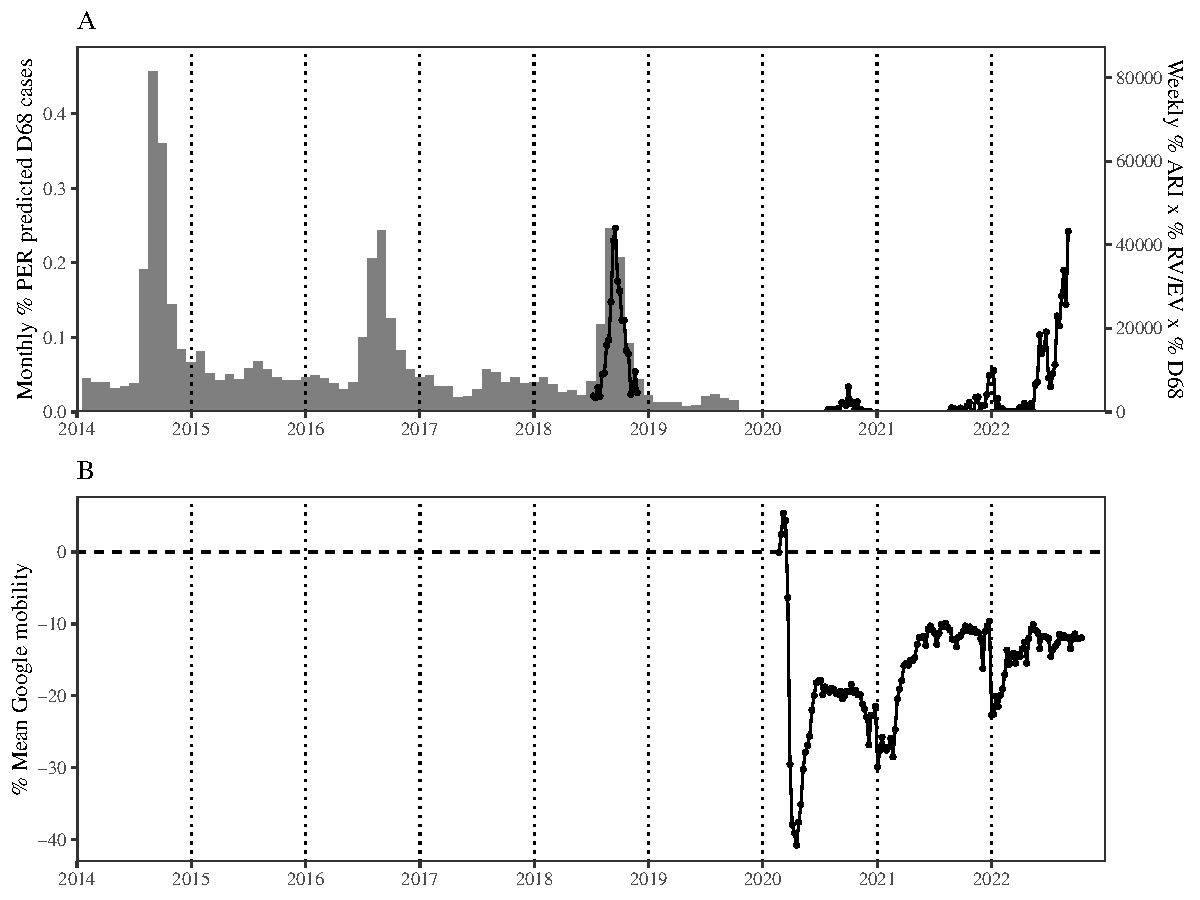
\includegraphics[width=\textwidth]{../figure_pub/figure1.pdf}
\caption{
\textbf{Estimated incidence proxy for enterovirus D68 circulations and Google mobility during the pandemic period in the US.}
(A) Weekly incidence proxy for enterovirus D68 (black lines and point) calculated by multiplying (1) weekly percentages of ED visits associated with ARIs, (2) weekly percentages of RV/EV positives, and (3) weekly percentages of EV-D68 positives.
The data are digitized from the figure of \cite{ma2022increase}.
Gray bars represent monthly percentages of positives for EV-D68 in the US predicted by the Pathogen Extended Resolution (PER) algorithm through the BioFire Syndromic Trends (Trend) network.
The data are publicly available from \cite{park2021epidemiological}.
(B) Percent changes in mean Google mobility across for categories (retail \& recreation, grocery \& pharmacy, transit stations, and workplaces).
The data are publicly available from \url{https://ourworldindata.org/covid-google-mobility-trends}.
}
\label{fig:fig1}
\end{figure}

Prior to 2020, circulations of enterovirus D68 exhibited predominantly biennial patterns in the US (\fref{fig1}A) and in other countries.
Based on this data, we previously predicted a possibility of a large outbreak in 2020, following the biennial pattern, and further showed that the decreased contact rates due to NPIs for the COVID-19 pandemic could, as observed, prevent this EV-D68 outbreak \citep{park2021epidemiological}.
The estimated incidence proxy from the NVSN data \citep{ma2022increase} confirms our prediction: there were limited cases during 2020 followed by a large outbreak in 2022.
Using the ILI time series also gave similar incidence proxy estimates (Supplementary Figure S1).
Interestingly, we found signatures of continued reduction in mobility throughout 2022 (\fref{fig1}B), which likely affected the dynamics of EV-D68 and further contributed to delaying the timing of its resurgence.

\begin{figure}[!th]
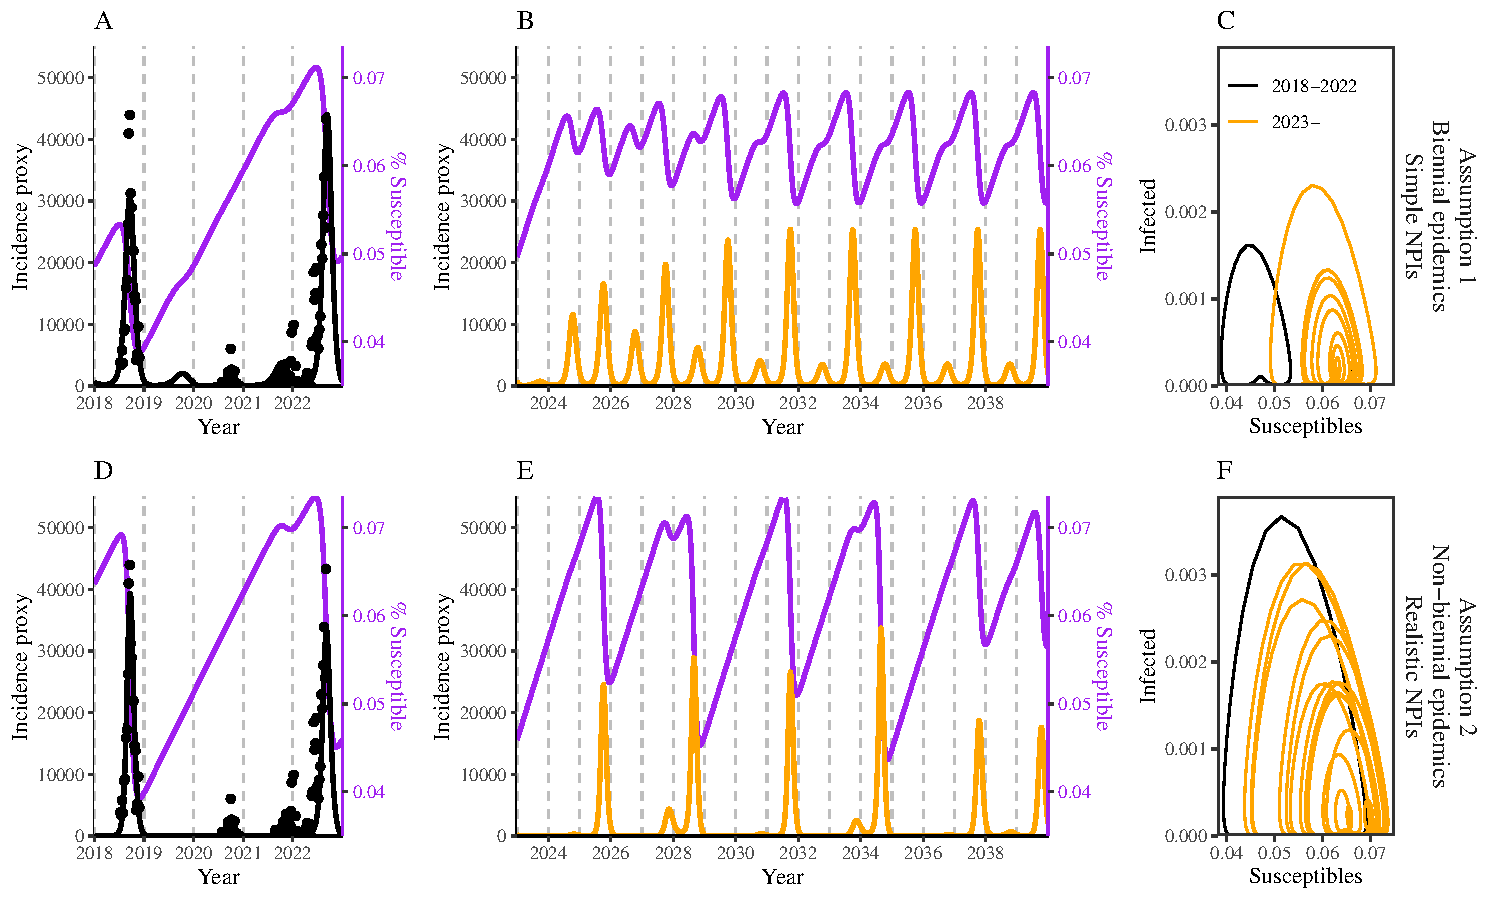
\includegraphics[width=\textwidth]{../figure_pub/figure2.pdf}
\caption{
\textbf{Model fits and long-term predictions under two different assumptions.}
(A,D) Fits of the SIR model (black lines) to incidence proxy (black points).
Purple lines represent the corresponding susceptible dynamics.
(B,E) Longer term predictions assuming a continued reduction in contact rates, which is modeled by either by fixing $\delta_2$ (assumption 1) or continuing the google mobility pattern (assumption 2).
(C,F) Phase diagram of prevalence of infection ($I/N$) against the proportion susceptible ($S/N$).
}
\label{fig:fig2}
\end{figure}

Under the first set of assumptions (endemic biennial circulation followed by step changes in contact rates), we estimated that a 28\% reduction in contact rates in 2020 and 2021, followed by a 24\% reduction in contact rates in 2022, provided the best fit to the observed dynamics (\fref{fig2}A).
In this case, the model predicts a slightly larger outbreak for 2022 than for 2018.
Consistent with the initial stable biennial assumption, the model predicts a return to stable biennial epidemic under a constant reduction in contact rates after 2022 (\fref{fig2}B);
the model also predicts an increase in the overall susceptibility compared to pre-pandemic periods (\fref{fig2}C).

The likelihood surface shows a strong correlation in two parameters (i.e., the amount of reduction in transmission in 2020--2021 vs 2022; Supplementary Figure S3), meaning that many other parameter combinations can give similar fits.
For example, a 40\% reduction followed by a 27\% reduction gives a very similar fit with $<2$ differences in log-likelihood units.
In Supplementary Figure S4, we present all model fits within 2 log-likelihood units compared to the best fit;
all of these model fits predict a return to stable biennial epidemic.
Further constraining paramter uncertainties would require detailed data on age-specific contact rates.
We were not able to find data on contact rates for age groups that are relevant to EV-D68 infections in the US (median of 2.9 vs 2.6 years for the 2018 and 2022 outbreak, respectively \citep{shah2021enterovirus,ma2022increase}).

Under the second set of assumptions (realistic changes in contact rates), we estimated $\mathcal R_0 =17.5$ and $\omega = 0.1$ best captures the observed dynamics (\fref{fig2}D; Supplementary Figure S5).
In this case, the model predicts a slightly larger outbreak for 2018 than for 2022.
Assuming a constant reduction in contact rates after 2022, the model predicts more complex longer-term oscillatory dynamics (\fref{fig2}E, \fref{fig2}F).

Two sets of assumptions gave similar log-likelihood estimates: -943.7 and -943.3, respectively.
QQ plots further indicated similarities in both fits (Supplementary Figure S6).
QQ plots indicated some deviation from the normal distribution towards the end of the quantiles;
these discrepancies were likely driven by systematic differences in the model predictions and data (e.g., underestimation of the 2018 peak for the assumption 1 and overestimation of 2022 peak for the assumption 2).
On the other hand, there was a considerable differences in the estimates of scaling parameter: 18.7 and 10.4, respectively.
We were not able to convert these scaling parameters to reporting probabilities given that the surveillance network only covers a relatively narrow region in the US.

Despite discrepant predictions in long-term dynamics across out modeling assumptions, the model predicts an absence of EV-D68 outbreak in 2023 under both sets of assumptions when there is a continued reduction in contact rates (\fref{fig2}A,D).
However, it is likely that the contact rates will return to normal, or may have already returned to normal values.
We therefore performed sensitivity analyses to characterize how short- and long-term predictions are sensitive to changes in future contact rates (\fref{fig3}).

\begin{figure}[!th]
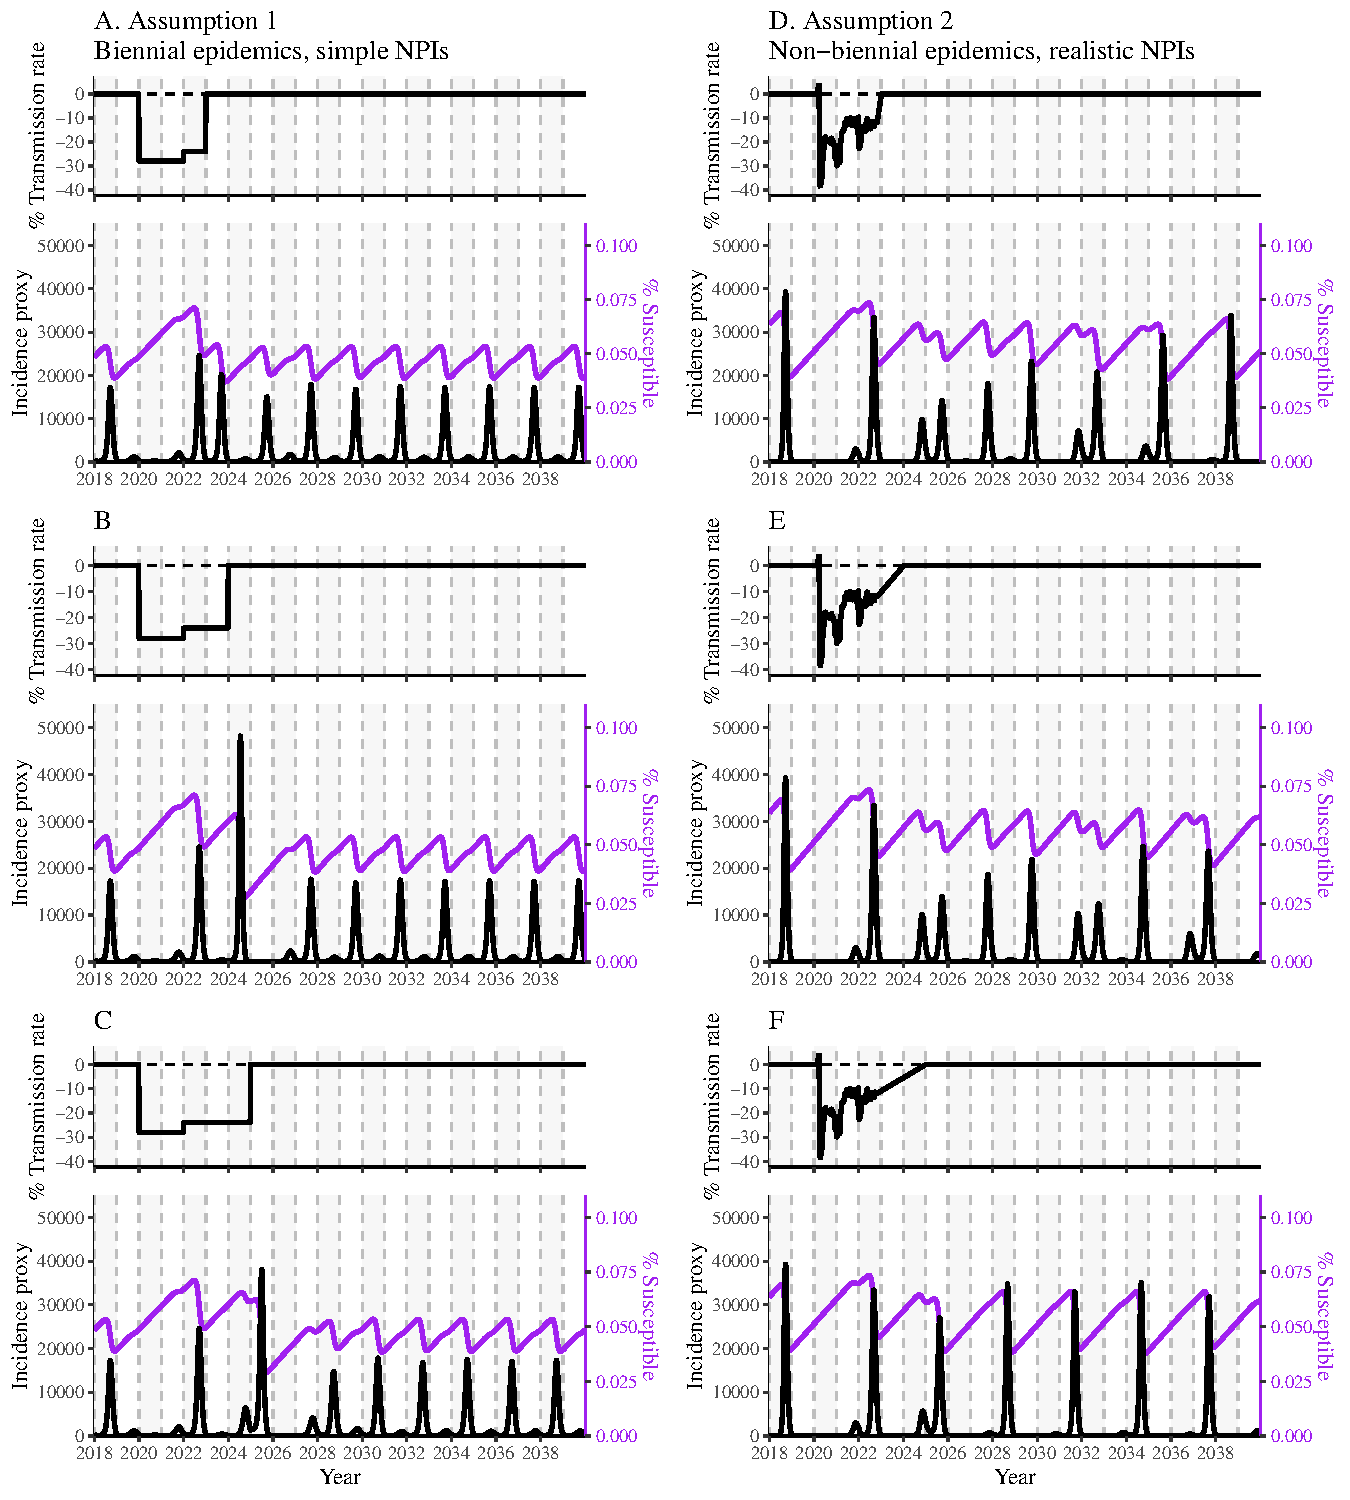
\includegraphics[width=\textwidth]{../figure_pub/figure3.pdf}
\caption{
\textbf{Sensitivity of long-term predictions to relaxations of changes in future contact rates.}
Top panels: assumed shape of the changes in contact rates $\delta(t)$ that were used to simulate the epidemics.
Bottom panels: model predictions.
Black lines represent the predicted incidence.
Purple lines represent the susceptible dynamics.
We assumed that contact rates will return to normal by the end of 2023 (A,D), 2024 (B,E), and 2025 (C,F).
}
\label{fig:fig3}
\end{figure}

Under the first set of assumptions, the model always predicts a stable biennial epidemic, but the short-term dynamics differ depending on how long it takes for contact rates to return to the pre-pandemic norm (\fref{fig3}A--C).
Specifically, we found that an outbreak in 2023 is possible if the contact rate had returned to normal by the beginning of 2023;
in all other scenarios, the model predicts no outbreak in 2023.
On the other hand, we found that the impact of changes in contact rates were less predictable under the second set of assumptions (\fref{fig3}D--F).
For example, when we assumed that the contact rates returned to normal by 2025, the predicted dynamics quickly converged to a 3 year cycle (\fref{fig3}F), which was not readily observed in other scenarios (\fref{fig3}D,E).

\section{Discussion}

In this study, we investigated the impact of COVID-19 NPIs on current and future dynamics of EV-D68 in the US.
Using published data from NVSN, we reconstructed an incidence proxy for EV-D68 infections and fitted the SIR model to the incidence proxy under two different assumptions about the underlying dynamics and the shape of NPIs.
For the first set of simulations, we assumed an underlying biennial epidemic and tried to estimate the shape of simple NPIs that would explain the observed dynamics.
For the second set of simulations, we allowed the underlying dynamics to deviate from the biennial epidemic but instead modeled the effects of NPIs using Google mobility measures.
We found that the observed dynamics can be explained under both sets of assumptions, but they predict markedly different long-term dynamics.
Both sets of simulations agree in predicting the absence of large outbreak for late 2023 in most scenarios.
This prediction follows intuitively from susceptible depletion following the large outbreak EV-D68 across the US.
However, the potential cannot be fully ruled out:
in particular, if the size of the EV-D68 outbreak in 2022 was offset by a moderate reduction in contact rates, thereby preventing a significant susceptible depletion, a sudden increase in contact between 2022 and 2023 can still cause an outbreak in 2023.
Serological surveys would help reduce uncertainties in both data and model predictions \citep{nguyen2022enterovirus}.

The two sets of assumptions that we considered represent different extremes.
The first captures the biennial patterns of EV-D68 outbreaks but makes simplifying assumptions about the impact of NPIs.
The second set of assumptions captures realistic changes in contact rates but does not account for the dynamics before 2018.
Given geographical heterogeneity in EV-D68 dynamics before 2018 and uncertanties in the exact changes in contact rates after the emergence of COVID-19, it is difficult to assess which assumptions are more realistic.
We tried combining a biennial pattern with realistic NPIs but such a combination gave significantly worse fits than two other assumptions.
Specifically, we tried to further relax the assumptions about realistic NPIs by modeling the changes in contact rates as a product of the mean Google mobility and a constant value, but the model consistently overestimated the size of 2021 outbreak and predicted a late outbreak for 2022 (see Supplementary Figure S7 for the fit).
Accounting for geographical heterogeneity in EV-D68 circulations and behavioral changes will be critical to making more accurate inferences and predictions;
such efforts would require us to fit our model at a finer geographical scale.
Overall, more detailed surveillance is required to better understand both short- and long-term dynamics of EV-D68.

There are many limitations to our analysis.
First of all, surveillance efforts for EV-D68 are currently limited in the US, adding large uncertainties to its observed dynamics.
Even though EV-D68 is thought to have circulated every two years before 2020, earlier analysis revealed large geographical heterogeneity in its patterns of spread.
Therefore, our estimated incidence proxy for the US provides a crude view of the overall dynamics and does not capture any geographical heterogeneity that may be present.
Second, we did not have access to the raw data and so we manually digitized the data.
This procedure likely added inaccuracies to the data (though this is likely not a major error).
Finally, our mathematical model necessarily relies on many simplifying assumptions that neglect age heterogeneities, immune and phylodynamic complexities, etc.
However, it would be impractical to try to fit more complicated models at this juncture, due to limited data.

There are considerable uncertainties in model parameters that we did not consider in our analysis.
Instead, we assumed that many parameters were known prior to model fits.
Nonetheless, our analysis already demonstrates that a wide range of scenarios are consistent with the observed dynamics, and
these scenarios give vastly different predictions.
Further exploring parameter spaces would provide a broader overview of potential epidemic trajectories, but our qualitative conclusion about the uncertainties around future dynamics would not change.

We modeled changes in EV-D68 transmission rates during the pandemic period using Google mobility, but there are many limitations to this approach.
Most importantly, Google mobility captures the behavior of mobile phone users (older age groups), whereas EV-D68 primarily infects considerably young children (3--4 years).
In other words, Google mobility would be a poor proxy for EV-D68 transmisison if there are systematic differences in contact patterns between younger and older age groups.
Using national mobility further neglects geographical heterogeneity in EV-D68 dynamics and surveillance efforts.
Age- and region-specific data are needed to better understand the changes in EV-D68 transmission during the NPI periods.

Given the uncoupling of EV-D68 circulation with AFM cases in 2022, uncertainty remains about the frequency of AFM cases associated with future outbreaks of particular strains of EV-D68.
It is unclear at this time whether changes in the virus, changes in host immunity, or both caused the apparent lack of AFM in 2022 despite the large EV-D68 outbreak.
For example, EV-D68 strains that circulated in 2022 are broadly similar to those in 2018, but even small changes in the virus can lead to large changes in neurovirulence.
On the other hand, an increase in the susceptible pool during the pandemic could have also caused an increase in the mean age of infection of EV-D68 in 2022, which may lead to less severe infections.
A coupling of molecular epidemiology and detailed surveillance data, such as age-structured surveillance or serological surveys, may provide better power to test different hypotheses and understand the relationship between AFM and EV-D68.
Further extending the analysis to EV-D68 outbreak dynamics in other countries and massive natural experiments of parallel impacts of COVID-19 NPI measures to dynamics of other endemic viral infections is critical \citep{baker2020impact}.

\section*{Data availability}

All data and code are stored in a publicly available GitHub repository (\url{https://github.com/parksw3/enteronpi}).


\section*{Acknowledgements}

We thank the NIH, VRC, PREMISE Program, Claire Midgley, Janell A. Routh, and Heidi Moline for help and discussions.
We thank the New Vaccine Surveillance Network (NVSN) for generating, and providing summaries of, key EV-D68 surveillance data.

\pagebreak

\section*{Supplementary Materials}
\setcounter{figure}{0}
\renewcommand{\thefigure}{S\arabic{figure}}

\begin{figure}[!th]
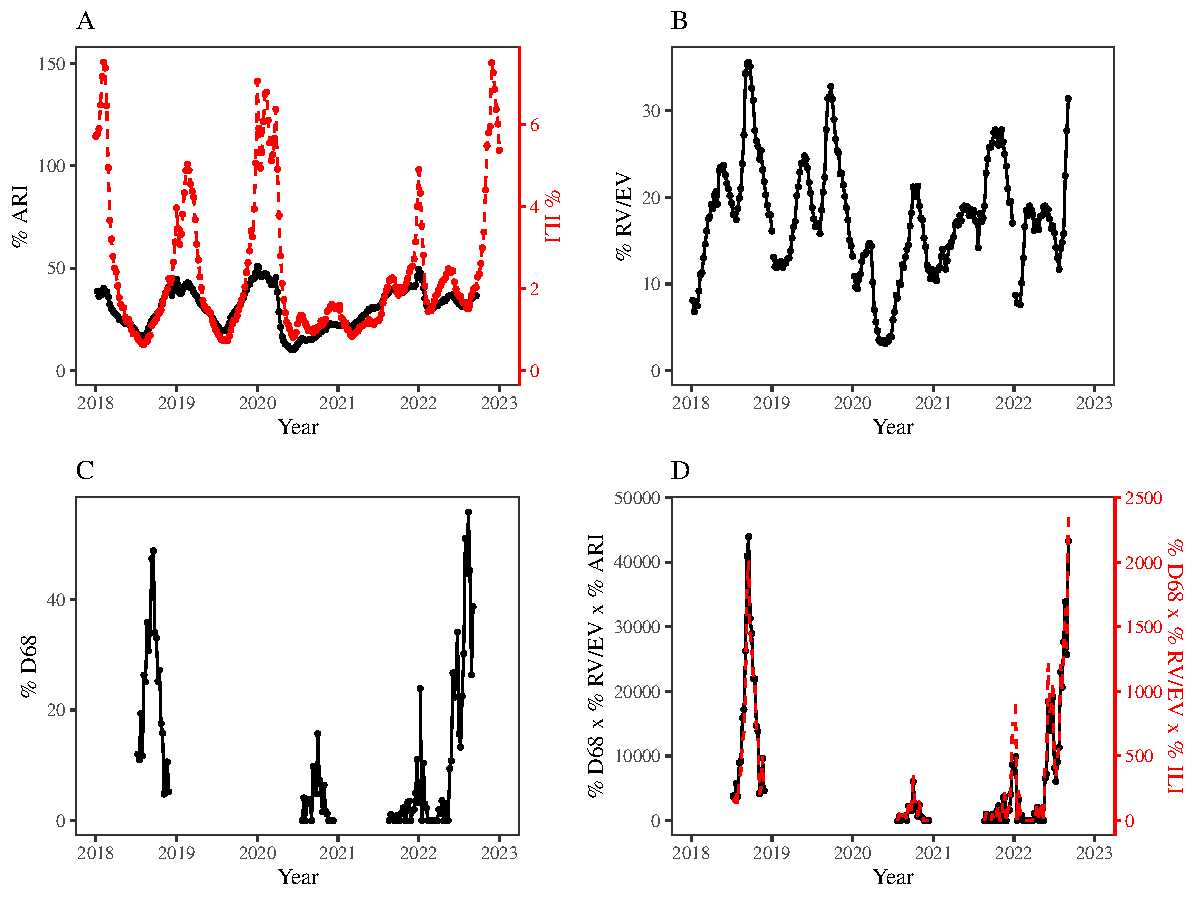
\includegraphics[width=\textwidth]{../figure_pub/figure_data_processed_d68.pdf}
\caption{
\textbf{Time series representing circulations of respiratory diseases and EV-D68.}
(A) Weekly percentages of ED visits for children and adolescents (<18 years old) associated with ARIs (black) and the weekly proportions of ILI visits (red).
(B) Weekly percentages of positives for rhinovirus and enterovirus.
(C) Weekly percentages of positives for EV-D68 among RV/EV positives.
(D) Weekly incidence proxy estimated using ARIs (black) and ILI (red) time series.
}
\end{figure}

\pagebreak

\begin{figure}[!th]
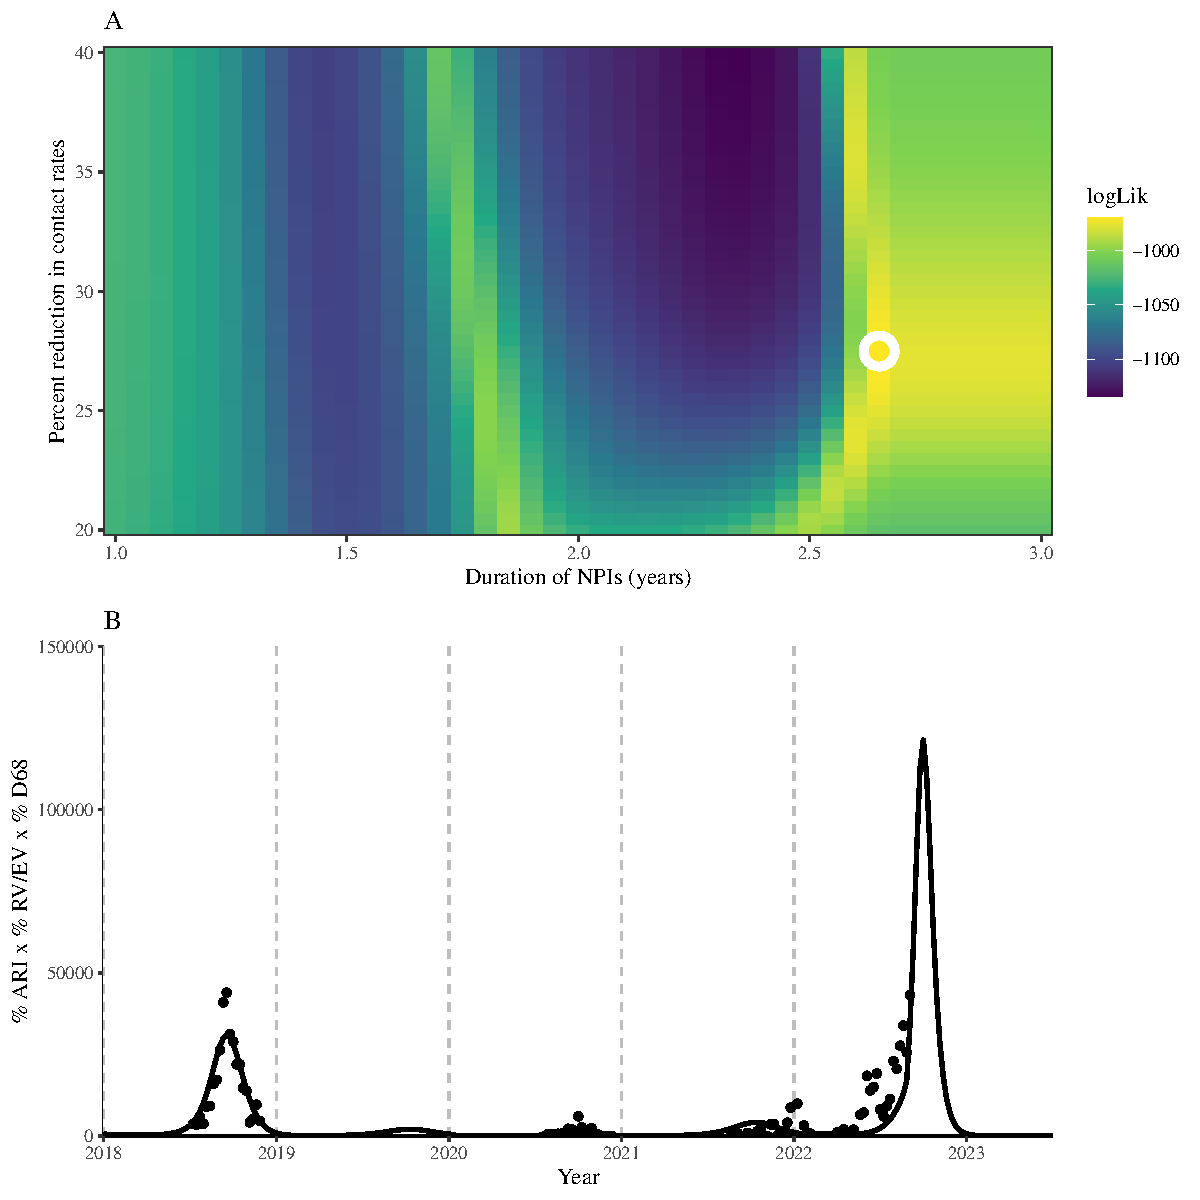
\includegraphics[width=\textwidth]{../figure_pub/figure_fit_npi_simple.pdf}
\caption{
\textbf{Results of fitting the SIR model with a constant reduction in contact rates over a fixed period.}
(A) The log likelihood surface of the model fits.
The circle represents the best fitting parameter.
(B) The best fit of the SIR model (black lines) to incidence proxy (black points).
}
\end{figure}

\pagebreak

\begin{figure}[!th]
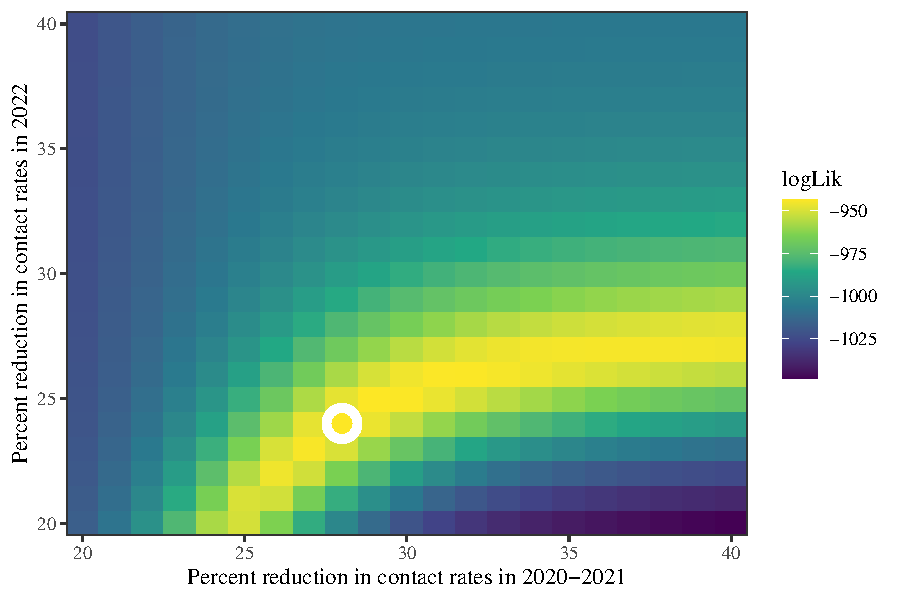
\includegraphics[width=\textwidth]{../figure_pub/figure2_logLik_1.pdf}
\caption{
\textbf{The log likelihood surface of the model fits under the first set of assumptions.}
The circle represents the best fitting parameter.
}
\end{figure}

\pagebreak

\begin{figure}[!th]
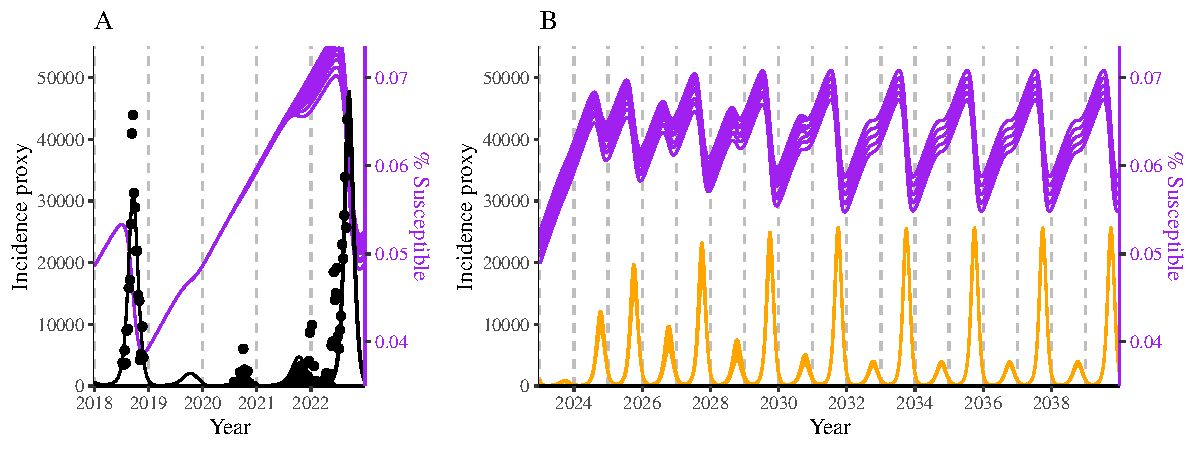
\includegraphics[width=\textwidth]{../figure_pub/figure2_alternative.pdf}
\caption{
\textbf{Uncertainties in model fits and long-term predictions under assumption 1.}
(A) Fits of the SIR model (black lines) to incidence proxy (black points).
Purple lines represent the corresponding susceptible dynamics.
(B) Longer term predictions assuming a continued reduction in contact rates, which is modeled fixing $\delta_2$.
Here, we present all model fits within 2 log-likelihood units compared to the best fit.
}
\end{figure}

\pagebreak

\begin{figure}[!th]
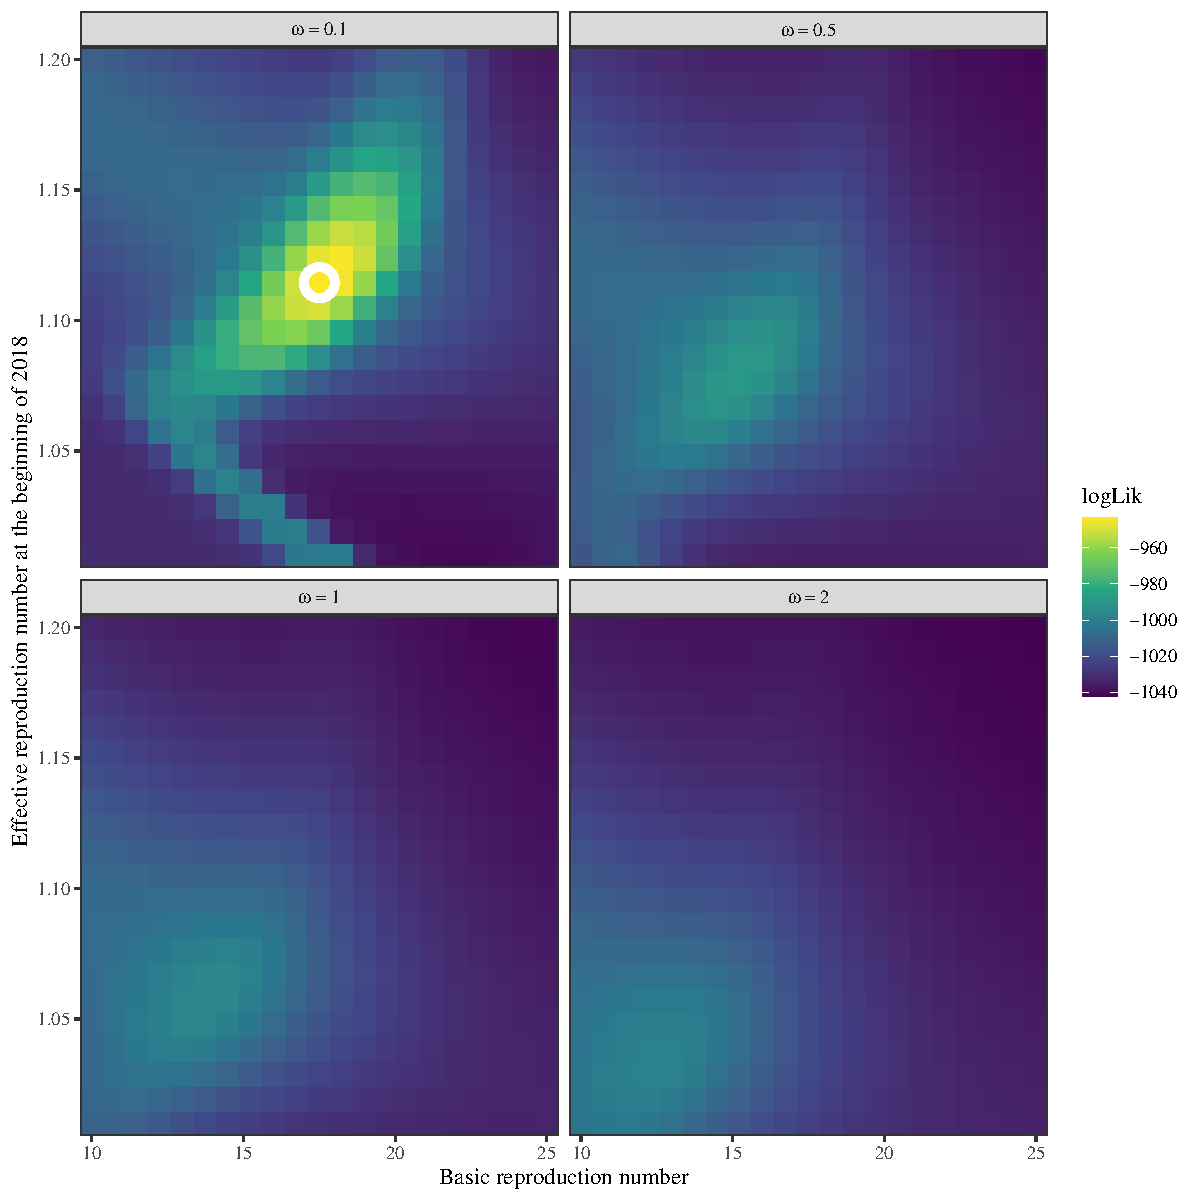
\includegraphics[width=\textwidth]{../figure_pub/figure2_logLik_2.pdf}
\caption{
\textbf{The log likelihood surface of the model fits under the second set of assumptions.}
The circle represents the best fitting parameter.
}
\end{figure}


\pagebreak

\begin{figure}[!th]
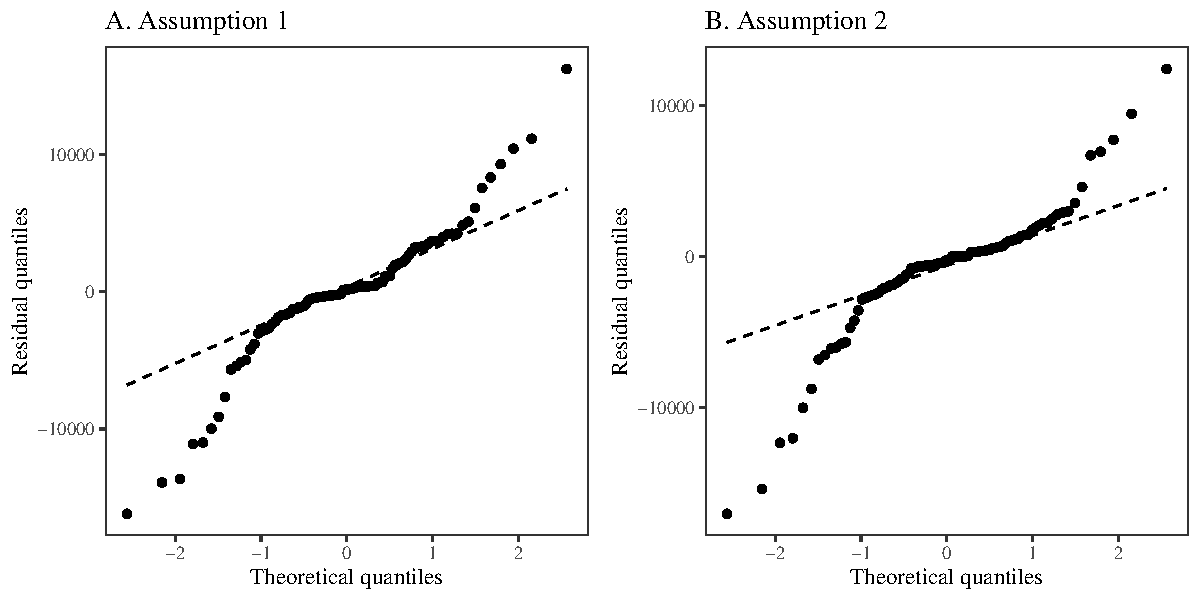
\includegraphics[width=\textwidth]{../figure_pub/figure2_qq.pdf}
\caption{
\textbf{QQ plots of residuals under two sets of assumptions against the quantiles of a standard normal quantiles.}
}
\end{figure}

\pagebreak

\begin{figure}[!th]
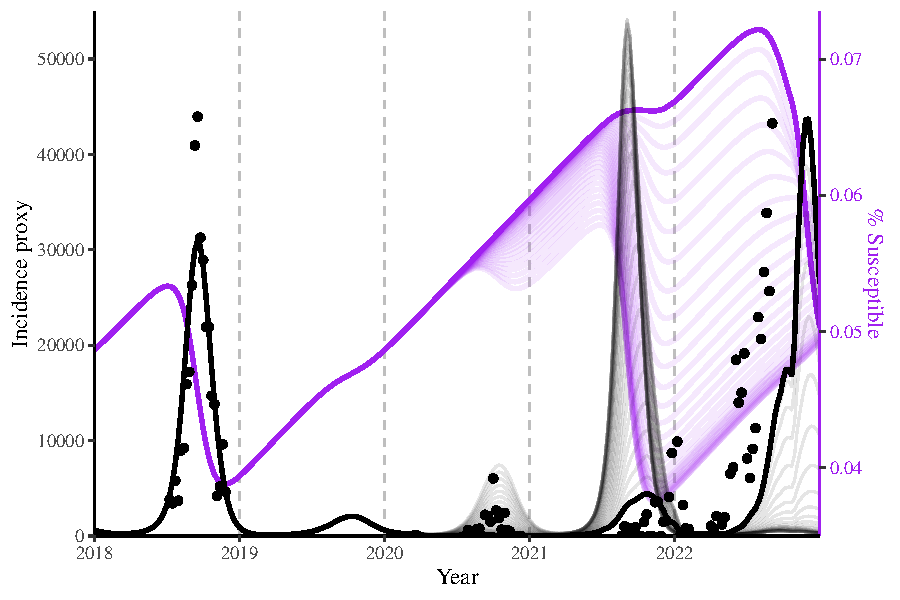
\includegraphics[width=\textwidth]{../figure_pub/figure2_biennial_mob.pdf}
\caption{
\textbf{Model fits and long-term predictions by assuming a biennial epidemic and using realistic NPIs.}
Fits of the SIR model (black lines) to incidence proxy (black points).
Purple lines represent the corresponding susceptible dynamics.
We modeled $\delta$ as a product of mean Google mobility and a constant value, ranging from 0.5 to 2.4.
We were not able to use a higher value for this mobility scaling constant because the reduction in transmission rate in 2020 would then exceed 100\%, thereby resulting in negative transmission rates.
Solid lines represent the best fits and lighter colors represent all other fits for different scaling factors.
}
\end{figure}


\pagebreak


\bibliography{enteronpi}

\end{document}
